\documentclass[a4paper,11pt,reqno]{amsart}

\usepackage[utf8]{inputenc}
\usepackage[foot]{amsaddr}
\usepackage{amsmath,amsfonts,amssymb,amsthm,mathrsfs,bm}
\usepackage[margin=0.95in]{geometry}
\usepackage{color}
\usepackage[dvipsnames]{xcolor}

\usepackage{etoolbox}

% Modifications to amsart ToC-related macros...
\makeatletter
\let\old@tocline\@tocline
\let\section@tocline\@tocline
% Insert a dotted ToC-line for \subsection and \subsubsection only
\newcommand{\subsection@dotsep}{4.5}
\newcommand{\subsubsection@dotsep}{4.5}
\patchcmd{\@tocline}
  {\hfil}
  {\nobreak
     \leaders\hbox{$\m@th
        \mkern \subsection@dotsep mu\hbox{.}\mkern \subsection@dotsep mu$}\hfill
     \nobreak}{}{}
\let\subsection@tocline\@tocline
\let\@tocline\old@tocline

\patchcmd{\@tocline}
  {\hfil}
  {\nobreak
     \leaders\hbox{$\m@th
        \mkern \subsubsection@dotsep mu\hbox{.}\mkern \subsubsection@dotsep mu$}\hfill
     \nobreak}{}{}
\let\subsubsection@tocline\@tocline
\let\@tocline\old@tocline

\let\old@l@subsection\l@subsection
\let\old@l@subsubsection\l@subsubsection

\def\@tocwriteb#1#2#3{%
  \begingroup
    \@xp\def\csname #2@tocline\endcsname##1##2##3##4##5##6{%
      \ifnum##1>\c@tocdepth
      \else \sbox\z@{##5\let\indentlabel\@tochangmeasure##6}\fi}%
    \csname l@#2\endcsname{#1{\csname#2name\endcsname}{\@secnumber}{}}%
  \endgroup
  \addcontentsline{toc}{#2}%
    {\protect#1{\csname#2name\endcsname}{\@secnumber}{#3}}}%

% Handle section-specific indentation and number width of ToC-related entries
\newlength{\@tocsectionindent}
\newlength{\@tocsubsectionindent}
\newlength{\@tocsubsubsectionindent}
\newlength{\@tocsectionnumwidth}
\newlength{\@tocsubsectionnumwidth}
\newlength{\@tocsubsubsectionnumwidth}
\newcommand{\settocsectionnumwidth}[1]{\setlength{\@tocsectionnumwidth}{#1}}
\newcommand{\settocsubsectionnumwidth}[1]{\setlength{\@tocsubsectionnumwidth}{#1}}
\newcommand{\settocsubsubsectionnumwidth}[1]{\setlength{\@tocsubsubsectionnumwidth}{#1}}
\newcommand{\settocsectionindent}[1]{\setlength{\@tocsectionindent}{#1}}
\newcommand{\settocsubsectionindent}[1]{\setlength{\@tocsubsectionindent}{#1}}
\newcommand{\settocsubsubsectionindent}[1]{\setlength{\@tocsubsubsectionindent}{#1}}

% Handle section-specific formatting and vertical skip of ToC-related entries
% \@tocline{<level>}{<vspace>}{<indent>}{<numberwidth>}{<extra>}{<text>}{<pagenum>}
\renewcommand{\l@section}{\section@tocline{1}{\@tocsectionvskip}{\@tocsectionindent}{}{\@tocsectionformat}}%
\renewcommand{\l@subsection}{\subsection@tocline{1}{\@tocsubsectionvskip}{\@tocsubsectionindent}{}{\@tocsubsectionformat}}%
\renewcommand{\l@subsubsection}{\subsubsection@tocline{1}{\@tocsubsubsectionvskip}{\@tocsubsubsectionindent}{}{\@tocsubsubsectionformat}}%
\newcommand{\@tocsectionformat}{}
\newcommand{\@tocsubsectionformat}{}
\newcommand{\@tocsubsubsectionformat}{}
\expandafter\def\csname toc@1format\endcsname{\@tocsectionformat}
\expandafter\def\csname toc@2format\endcsname{\@tocsubsectionformat}
\expandafter\def\csname toc@3format\endcsname{\@tocsubsubsectionformat}
\newcommand{\settocsectionformat}[1]{\renewcommand{\@tocsectionformat}{#1}}
\newcommand{\settocsubsectionformat}[1]{\renewcommand{\@tocsubsectionformat}{#1}}
\newcommand{\settocsubsubsectionformat}[1]{\renewcommand{\@tocsubsubsectionformat}{#1}}
\newlength{\@tocsectionvskip}
\newcommand{\settocsectionvskip}[1]{\setlength{\@tocsectionvskip}{#1}}
\newlength{\@tocsubsectionvskip}
\newcommand{\settocsubsectionvskip}[1]{\setlength{\@tocsubsectionvskip}{#1}}
\newlength{\@tocsubsubsectionvskip}
\newcommand{\settocsubsubsectionvskip}[1]{\setlength{\@tocsubsubsectionvskip}{#1}}

% Adjust section-specific ToC-related macros to have a fixed-width numbering framework
\patchcmd{\tocsection}{\indentlabel}{\makebox[\@tocsectionnumwidth][l]}{}{}
\patchcmd{\tocsubsection}{\indentlabel}{\makebox[\@tocsubsectionnumwidth][l]}{}{}
\patchcmd{\tocsubsubsection}{\indentlabel}{\makebox[\@tocsubsubsectionnumwidth][l]}{}{}

% Allow for section-specific page numbering format of ToC-related entries
\newcommand{\@sectypepnumformat}{}
\renewcommand{\contentsline}[1]{%
  \expandafter\let\expandafter\@sectypepnumformat\csname @toc#1pnumformat\endcsname%
  \csname l@#1\endcsname}
\newcommand{\@tocsectionpnumformat}{}
\newcommand{\@tocsubsectionpnumformat}{}
\newcommand{\@tocsubsubsectionpnumformat}{}
\newcommand{\setsectionpnumformat}[1]{\renewcommand{\@tocsectionpnumformat}{#1}}
\newcommand{\setsubsectionpnumformat}[1]{\renewcommand{\@tocsubsectionpnumformat}{#1}}
\newcommand{\setsubsubsectionpnumformat}[1]{\renewcommand{\@tocsubsubsectionpnumformat}{#1}}
\renewcommand{\@tocpagenum}[1]{%
  \hfill {\mdseries\@sectypepnumformat #1}}

% Small correction to Appendix, since it's still a \section which should be handled differently
\let\oldappendix\appendix
\renewcommand{\appendix}{%
  \leavevmode\oldappendix%
  \addtocontents{toc}{%
    \protect\settowidth{\protect\@tocsectionnumwidth}{\protect\@tocsectionformat\sectionname\space}%
    \protect\addtolength{\protect\@tocsectionnumwidth}{2em}}%
}
\makeatother

% #1 (default is as required)

% #2

% #3
\makeatletter
\settocsectionnumwidth{2em}
\settocsubsectionnumwidth{2.5em}
\settocsubsubsectionnumwidth{3em}
\settocsectionindent{1pc}%
\settocsubsectionindent{\dimexpr\@tocsectionindent+\@tocsectionnumwidth}%
\settocsubsubsectionindent{\dimexpr\@tocsubsectionindent+\@tocsubsectionnumwidth}%
\makeatother

% #4 & #5
\settocsectionvskip{10pt}
\settocsubsectionvskip{0pt}
\settocsubsubsectionvskip{0pt}

% #6 & #7
% See #3

% #8
\renewcommand{\contentsnamefont}{\bfseries\Large}

% #9
\settocsectionformat{\bfseries}
\settocsubsectionformat{\mdseries}
\settocsubsubsectionformat{\mdseries}
\setsectionpnumformat{\bfseries}
\setsubsectionpnumformat{\mdseries}
\setsubsubsectionpnumformat{\mdseries}

% #10
% Insert the following command inside your text where you want the ToC to have a page break
\newcommand{\tocpagebreak}{\leavevmode\addtocontents{toc}{\protect\clearpage}}

% #11
\let\oldtableofcontents\tableofcontents
\renewcommand{\tableofcontents}{%
  \vspace*{-\linespacing}% Default gap to top of CONTENTS is \linespacing.
  \oldtableofcontents}

\usepackage{mathtools,enumerate,mathrsfs,graphicx}
\usepackage{epstopdf}
\usepackage{hyperref}

\usepackage{latexsym}


\definecolor{CommentGreen}{rgb}{0.0,0.4,0.0}
\definecolor{Background}{rgb}{0.9,1.0,0.85}
\definecolor{lrow}{rgb}{0.914,0.918,0.922}
\definecolor{drow}{rgb}{0.725,0.745,0.769}

\usepackage{listings}
\usepackage{textcomp}
\lstloadlanguages{Matlab}%
\lstset{
    language=Matlab,
    upquote=true, frame=single,
    basicstyle=\small\ttfamily,
    backgroundcolor=\color{Background},
    keywordstyle=[1]\color{blue}\bfseries,
    keywordstyle=[2]\color{purple},
    keywordstyle=[3]\color{black}\bfseries,
    identifierstyle=,
    commentstyle=\usefont{T1}{pcr}{m}{sl}\color{CommentGreen}\small,
    stringstyle=\color{purple},
    showstringspaces=false, tabsize=5,
    morekeywords={properties,methods,classdef},
    morekeywords=[2]{handle},
    morecomment=[l][\color{blue}]{...},
    numbers=none, firstnumber=1,
    numberstyle=\tiny\color{blue},
    stepnumber=1, xleftmargin=10pt, xrightmargin=10pt
}

\numberwithin{equation}{section}
\synctex=1

\hypersetup{
    unicode=false, pdftoolbar=true, 
    pdfmenubar=true, pdffitwindow=false, pdfstartview={FitH}, 
    pdftitle={ELE2024 Coursework}, pdfauthor={A. Author},
    pdfsubject={ELE2024 coursework}, pdfcreator={A. Author},
    pdfproducer={ELE2024}, pdfnewwindow=true,
    colorlinks=true, linkcolor=red,
    citecolor=blue, filecolor=magenta, urlcolor=cyan
}


% CUSTOM COMMANDS
\renewcommand{\Re}{\mathbf{re}}
\renewcommand{\Im}{\mathbf{im}}
\newcommand{\R}{\mathbb{R}}
\newcommand{\N}{\mathbb{N}}
\newcommand{\C}{\mathbb{C}}
\newcommand{\lap}{\mathscr{L}}
\newcommand{\dd}{\mathrm{d}}
\newcommand{\smallmat}[1]{\left[ \begin{smallmatrix}#1 \end{smallmatrix} \right]}

%opening
\title[MATH 2860 (Elementary Differential Equations)]{Homework 1 for MATH 2860 (Elementary Differential Equations)}

\author[Emmanuel Atindama]{E. A. Atindama, PhD Mathematics}

\address[E. A. Atindama]{. Email addresses: \href{emmanuel.atindama@utoledo.edu}{emmanuel.atindama@utoledo.edu} 
% and 
% \href{mailto:a.student@qub.ac.uk}{a.student@qub.ac.uk}.
}
\thanks{Version 0.0.1. Last updated:~\today.}

\begin{document}

\maketitle






\subsection*{Question Q1}
\begin{enumerate}[a)]
    \item Construct a slope field of the differential equation
        \[
        y' = -\frac{x}{y}
        \]
    for \(y=-3, -2, -1, 0, 1, 2, 3\) and your own choice of \(x-\)values.  
    \item From your slope field, \textbf{sketch} one integral curve.
\end{enumerate}

\begin{center}\setlength{\fboxsep}{10pt}\fcolorbox{yellow!20}{yellow!20}{\parbox{0.9\linewidth}{
\textbf{Solution}

    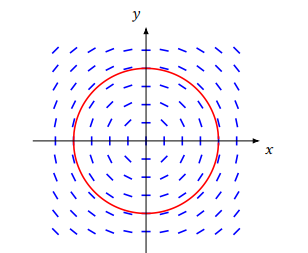
\includegraphics[width=0.7\linewidth]{../figs/h1_q1.png}

    The solution to part (a) is the blue ticks only. The solution to part (b) is the red circle.
}}
\end{center}



\subsection*{Question Q2}
    Find the solution to the differential equation
    \[
    y' = \frac{1}{x^2 + x}; \: y(0) = 1.
    \]
   In other words, integrate the function \(y'\).

\begin{center}\setlength{\fboxsep}{10pt}\fcolorbox{yellow!20}{yellow!20}{\parbox{0.9\linewidth}{
\textbf{Solution}

We can integrate \(y'=\dfrac{1}{x^2+x}\) by partial fractions, but the initial condition at \(x=0\) is problematic.

\[
\frac{1}{x^2+x}=\frac{1}{x(x+1)}=\frac{1}{x}-\frac{1}{x+1}.
\]

Hence

\[
y(x)=\int\!\left(\frac{1}{x}-\frac{1}{x+1}\right)\,dx
= \ln|x|-\ln|x+1|+C
= \ln\!\left|\frac{x}{x+1}\right|+C,
\qquad (x\neq 0,-1).
\]


The differential equation is \textbf{not defined at} \(x=0\) (the right-hand side blows up), and

\[
\lim_{x\to 0}\left(\ln|x|-\ln|x+1|+C\right)=-\infty
\]

for any constant $C$. Therefore it is **impossible** to choose \(C\) so that \(y(0)=1\).

The general solution (on any interval avoiding \(x=0\) and \(x=-1\)) is

\[
\boxed{\,y(x)=\ln\!\left|\frac{x}{x+1}\right|+C\,}
\]

\(\lim_{x\to 0}y(x)=-\infty\). Thus \textbf{the IVP has no solution}.
}}
\end{center}



\subsection{Question Q3}
    \begin{enumerate}[a)]
        \item Which of the following is the general solution to the differential equation
            \[
            y' -2y +e^x = 0.
            \]
           \begin{enumerate}[i)]
               \item \(y = ce^{2x} + x\)
               \item \(y = ce^{2x} + e^{-x}\)
               \item \(y = ce^{x} + e^{-x}\)
               \item \(y = e^x - ce^{2x} \)
           \end{enumerate}
       \item From your answer in (a), solve the IVP
            \[
            y' -2y +e^x = 0, \: y(0) = 2.
            \]
    \end{enumerate}


\begin{center}\setlength{\fboxsep}{10pt}\fcolorbox{yellow!20}{yellow!20}{\parbox{0.9\linewidth}{
\textbf{Solution}

I’ll show the derivative and the substitution for each option to determine which satisfies the differential equation.

\begin{enumerate}[i)]
    \item \(y = c e^{2x} + x \Rightarrow  y' = 2c e^{2x} + 1 \)
    
    Substitute:
    
    \[
    y' - 2y + e^x
    = (2c e^{2x} + 1) - 2(c e^{2x} + x) + e^x
    = 1 - 2x + e^x \quad \text{not a solution}.
    \]

    
    \item \(y = c e^{2x} + e^{-x} \Rightarrow y' = 2c e^{2x} - e^{-x}\)
    
    Substitute:
    
    \[
    y' - 2y + e^x
    = \big(2c e^{2x} - e^{-x}\big) - 2\big(c e^{2x} + e^{-x}\big) + e^x
    = -3e^{-x} + e^x, \quad \text{not a solution}
    \]
\end{enumerate}
}}
\end{center}    

\begin{center}\setlength{\fboxsep}{10pt}\fcolorbox{yellow!20}{yellow!20}{\parbox{0.9\linewidth}{

\begin{enumerate}
    \item[iii)] \(y = c e^{x} + e^{-x} \Rightarrow y' = c e^{x} - e^{-x}\)
    
    Substitute:
    
    \[
    y' - 2y + e^x
    = (c e^{x} - e^{-x}) - 2(c e^{x} + e^{-x}) + e^x
    = (1-c)e^{x} - 3e^{-x},
    \quad \text{not a solution}
    \]
    
    
    
    \item[iv)] \(y = e^x - c e^{2x} \Rightarrow y' = e^x - 2c e^{2x} \)
    
    Substitute:
    
    \[
    y' - 2y + e^x
    = (e^x - 2c e^{2x}) - 2(e^x - c e^{2x}) + e^x
    = e^x -2c e^{2x} -2e^x +2c e^{2x} + e^x
    = 0.
    \]
    
    \textbf{Therefore (iv) is a valid general solution} (\(y=e^x + C e^{2x}\) with \(C=-c\)).

\end{enumerate}

\vspace{1cm}

Part (b): Solve the IVP \(y' - 2y + e^x = 0,\; y(0)=2\)

Use the valid form \(y(x)=e^x - c e^{2x}\). Apply the initial condition \(x=0\):

\[
y(0)= e^0 - c e^{0} = 1 - c = 2 \quad\Rightarrow\quad c = -1.
\]

Thus the particular solution is

\[
\boxed{\,y(x)=e^x + e^{2x}\,}
\]

---

The correct option is (iv).
The solution of the IVP is \(\; y(x)=e^x + e^{2x}.\)
}}
\end{center}


\end{document}
